\documentclass[12pt,a4paper]{report}

% Paquetes
\usepackage[utf8]{inputenc}
\usepackage[T1]{fontenc}
\usepackage[english]{babel}
\usepackage{lmodern}
\usepackage[numbers,sort&compress]{natbib}
\usepackage{placeins,float}
\newenvironment{resulttable}{\begin{table}[!htbp]}{\end{table}}
\renewcommand{\chaptername}{Capítulo}
\renewcommand{\tablename}{Tabla}
\renewcommand{\figurename}{Figura}
\renewcommand{\contentsname}{Contenido}
\renewcommand{\bibname}{Referencias}
\addto\captionsenglish{\renewcommand{\chaptername}{Capítulo}\renewcommand{\tablename}{Tabla}\renewcommand{\figurename}{Figura}\renewcommand{\contentsname}{Contenido}\renewcommand{\bibname}{Referencias}}
\usepackage{amsmath,amssymb}
\usepackage{graphicx}
\usepackage{booktabs}
\usepackage{array}
\usepackage{longtable}
\usepackage[margin=1in]{geometry}
\usepackage[hidelinks]{hyperref}
\usepackage{xcolor}
\usepackage{listings}
\usepackage{url}

% Configuración
\setlength{\parskip}{0.5em}
\setlength{\parindent}{0pt}
\setlength{\tabcolsep}{5pt}

% Título
\title{\textbf{Concatenación sistemática de descriptores visuales clásicos y modernos para clasificación de texturas} \\
\large Evaluación anidada de estrategias de concatenación de 21 descriptores}
\author{Carlos Ayala \and Joaquín Delgado}
\date{Septiembre 2026}

\begin{document}

\maketitle

% ============================================================
% PORTADA
% ============================================================
\begin{titlepage}
\begin{center}
\vspace*{2cm}
{\Large \textbf{Universidad Nacional de Asunción}} \\
\vspace{0.3cm}
{\large Facultad Politécnica} \\
\vspace{2cm}
{\Huge \textbf{Concatenación sistemática de descriptores visuales clásicos y modernos para clasificación de texturas}} \\
\vspace{0.5cm}
{\large Evaluación anidada de estrategias de concatenación de 21 descriptores} \\
\vspace{3cm}
{\large \textbf{Carlos Ayala} \\
\textbf{Joaquín Delgado}} \\
\vspace{1cm}
{\large Tutor: José Vázquez} \\
\vspace{2cm}
{\large Septiembre 2026}
\end{center}
\end{titlepage}

% ============================================================
% AGRADECIMIENTOS
% ============================================================
\chapter*{Agradecimientos}
A nuestro tutor, José Vázquez, por su guía y paciencia. \\
A la Facultad Politécnica de la UNA, por el espacio y los recursos. \\
A nuestras familias, por el apoyo incondicional.

% ============================================================
% RESUMEN
% ============================================================
\chapter*{Resumen}

Este trabajo evalúa la concatenación de descriptores heterogéneos para clasificar texturas. Se comparan cinco estrategias: Individual, Completa, Top-$k$, Greedy Forward Selection (GFS) y Homogénea. La biblioteca evaluada reúne 21 descriptores sobre DTD, FMD, CUReT y Outex con SVM lineal y ResMLP. La selección se realiza dentro del entrenamiento y el desempeño se mide mediante macro-F1 y exactitud en 56 condiciones externas en total. GFS obtiene mayor macro-F1 medio que Individual en las ocho configuraciones dataset--clasificador, pero el método con mayor desempeño varía entre dominios y clasificadores. Con un bloque por dataset, Friedman ($p=0{,}1074$) y Quade ($p=0{,}0705$) no rechazan la hipótesis global, y ninguna comparación por pares resulta significativa tras Holm a $\alpha=0{,}05$. GFS reduce la dimensión media entre 71,7\% y 85,4\% respecto de la concatenación completa. Los resultados respaldan evaluar la composición y el costo dimensional según el dominio, sin establecer una estrategia universalmente superior.

\textbf{Palabras clave:} clasificación de texturas, concatenación de descriptores, selección de bloques, GFS, evaluación anidada.

\chapter*{Abstract}

This thesis compares five descriptor selection and concatenation strategies using 21 descriptors. The complete evaluation covers DTD, FMD, CUReT and Outex with linear SVM and a residual MLP, using 56 external conditions. GFS obtains higher mean macro-F1 than the internally selected individual descriptor in all eight dataset--classifier configurations. With one block per dataset, Friedman (p=0.1074) and Quade (p=0.0705) do not reject their global null hypotheses; no pairwise comparison is significant after Holm adjustment at 0.05. These results support evaluating concatenation by domain, performance and representation size, without establishing universal superiority.

\textbf{Keywords:} texture classification, descriptor concatenation, block selection, GFS, nested evaluation.

% ============================================================
% ÍNDICE
% ============================================================
\tableofcontents
\newpage

% ============================================================
% CAPÍTULOS
% ============================================================
\chapter{Introducción}\label{sec:introduccion}

La clasificación de texturas depende de señales locales, distribuciones espaciales y respuestas en frecuencia que cambian con el dominio, la escala, la iluminación y el punto de vista \citep{cimpoi2014dtd,cimpoi2016fisher,liu2019survey}. Ninguna representación captura necesariamente todas esas variaciones. Los descriptores clásicos resumen propiedades diseñadas, como microestructuras, coocurrencias y gradientes \citep{ojala2002lbp,haralick1979glcm,dalal2005hog}; las redes convolucionales, los Transformers y los modelos autosupervisados producen características aprendidas con arquitecturas y objetivos de preentrenamiento diferentes \citep{he2016resnet,tan2019efficientnet,dosovitskiy2021vit,liu2021swin,oquab2024dinov2}. Esta diversidad crea una oportunidad para combinar representaciones, pero también introduce redundancia, escalas incompatibles y un aumento considerable de dimensionalidad.

La concatenación conserva la información de varios extractores y delega al clasificador la decisión sobre sus coordenadas. Agregaciones locales, Fisher vectors, bancos de filtros profundos y capas de codificación aprendida han mostrado que combinar respuestas puede mejorar el reconocimiento de texturas \citep{sanchez2013image,cimpoi2016fisher,zhang2017deepten}. Sin embargo, una mejora de la representación conjunta no demuestra que todos sus bloques sean necesarios ni que la complementariedad explique por sí sola el resultado. El mismo efecto puede aparecer al aumentar la dimensión o al reunir descriptores que ya son fuertes de manera individual.

Las arquitecturas de fusión y las combinaciones de representaciones motivan distinguir tres factores en la evaluación: calidad individual, cantidad de variables y composición del subconjunto. La distinción adquiere especial importancia en una biblioteca que reúne descriptores clásicos, CNN, Transformers y representaciones autosupervisadas o multimodales. La pregunta de estudio es \emph{cómo cambian el desempeño externo y la dimensionalidad al concatenar descriptores, frente a seleccionar uno individual, y qué aporta elegir la composición de esa concatenación}.

Para responder esta pregunta se evaluaron 21 descriptores sobre DTD, FMD, CUReT y Outex con SVM lineal y ResMLP. El mismo protocolo anidado compara cinco estrategias: Individual, Completa, Top-$k$, GFS y Homogénea. La comparación considera macro-F1 y exactitud, junto con la dimensión de las representaciones. Se completaron 28 condiciones externas por clasificador; cada una incluye las cinco estrategias sobre la misma biblioteca de 21 descriptores.

El trabajo aporta una comparación reproducible de estrategias de concatenación bajo particiones comunes, una evaluación no paramétrica entre datasets y una comparación del desempeño y la dimensionalidad de los subconjuntos seleccionados. GFS y Top-$k$ son procedimientos para elegir qué bloques concatenar dentro de esta comparación. El propósito es caracterizar las ganancias y los costos observados de combinar bloques, sin introducir un nuevo algoritmo de selección. La evidencia se interpreta atendiendo tanto a las diferencias observadas como a la incertidumbre estadística.

La tesis se organiza en seis capítulos: introducción, antecedentes, metodología, resultados, discusión y conclusión. El estudio anidado con cuatro datasets constituye la referencia actual. Los experimentos exploratorios previos se conservan en los materiales del proyecto y no se mezclan con sus contrastes estadísticos.

% ============================================================
% 2. TRABAJOS RELACIONADOS
% ============================================================

\newpage
\chapter{Trabajos relacionados}\label{sec:trabajos}

\section{Representaciones de textura}

Los descriptores de textura resumen señales distintas de una misma imagen: microestructuras (LBP), coocurrencias, orientación de gradientes y patrones en frecuencia \citep{haralick1979glcm,ojala2002lbp,dalal2005hog,mehta2016drlbp}. Las representaciones aprendidas introducen sesgos adicionales derivados de arquitecturas convolucionales, Transformers y objetivos de preentrenamiento supervisado, autosupervisado o multimodal \citep{he2016resnet,tan2019efficientnet,dosovitskiy2021vit,liu2021swin,caron2021dino,oquab2024dinov2,he2022mae,radford2021clip,zhai2023siglip}. Por ello, ningún extractor debe suponerse universalmente suficiente: vectores con distinto origen pueden contener información redundante, pero también señales complementarias aprovechables por un clasificador conjunto. Esta complementariedad, y no la comparación aislada entre arquitecturas, motiva la composición de bloques del presente estudio.

\section{Concatenación y selección de bloques}

La fusión de características combina información antes de la decisión final del clasificador. Una estrategia directa consiste en concatenar los vectores extraídos de una misma imagen. A diferencia de la fusión de decisiones, esta operación conserva explícitamente las coordenadas de cada representación y permite entrenar un único clasificador sobre el espacio conjunto. Su sencillez constituye una ventaja experimental: permite estudiar el efecto de combinar descriptores sin introducir un módulo de fusión altamente parametrizado. No obstante, el vector resultante crece con cada extractor incorporado y puede acumular escalas incompatibles, variables redundantes y dimensiones poco informativas.

Los Fisher vectors mostraron que la agregación de descriptores locales puede producir representaciones de alto rendimiento \citep{sanchez2013image}; en texturas, los bancos de filtros profundos combinaron activaciones convolucionales con agregación estadística \citep{cimpoi2016fisher} y DeepTEN integró una capa de codificación residual dentro de una arquitectura profunda \citep{zhang2017deepten}. Estos antecedentes muestran que reunir señales distintas puede mejorar la representación, pero no determinan si todos los componentes son necesarios cuando la biblioteca contiene extractores heterogéneos y congelados.

Los antecedentes citados motivan evaluar si una búsqueda secuencial supera a reunir los descriptores individualmente más fuertes bajo el mismo número de bloques. Por ello, este estudio compara esas políticas bajo las mismas particiones y separa la selección de la evaluación externa, como recomiendan los diseños wrapper y la evaluación anidada \citep{kohavi1997wrappers,guyon2003feature}. El foco no está en proponer otro extractor ni en atribuir el resultado a una arquitectura particular, sino en evaluar la \emph{concatenación de descriptores como problema de selección de bloques}, comparando su desempeño externo y dimensionalidad. Igualar el número de bloques no iguala las dimensiones ni permite aislar causalmente la complementariedad.

% ============================================================
% 3. METODO
% ============================================================

\newpage
\chapter{Método de concatenación y selección de descriptores}\label{sec:metodo}

\section{Representación conjunta y pregunta de estudio}

El estudio evalúa la concatenación como un problema de selección de bloques. Cada extractor transforma una imagen $x_i$ en un vector $\mathbf{z}_{ij}\in\mathbb{R}^{d_j}$, donde $j$ identifica el descriptor y $d_j$ su dimensionalidad. Para un subconjunto $S$ de extractores, la representación conjunta se define como
\begin{equation}
 \mathbf{z}_{i,S}=\mathop{\Vert}_{j\in S}\frac{\mathbf{z}_{ij}}{\max(\lVert\mathbf{z}_{ij}\rVert_2,10^{-12})},
 \label{eq:concat}
\end{equation}
donde $\Vert$ denota concatenación. La normalización $L_2$ se aplica por descriptor y por muestra antes de unir los bloques, para evitar que la escala de un extractor determine por sí sola la contribución al clasificador.

La Figura~\ref{fig:pipeline} muestra cómo una misma imagen produce representaciones diferentes. Un descriptor resume patrones, relaciones entre intensidades o activaciones aprendidas en un vector. Después de normalizar cada bloque, se conserva un descriptor individual o se concatenan los bloques seleccionados. La dimensión conjunta es $d_S=\sum_{j\in S}d_j$.

\begin{figure}[!ht]
\centering
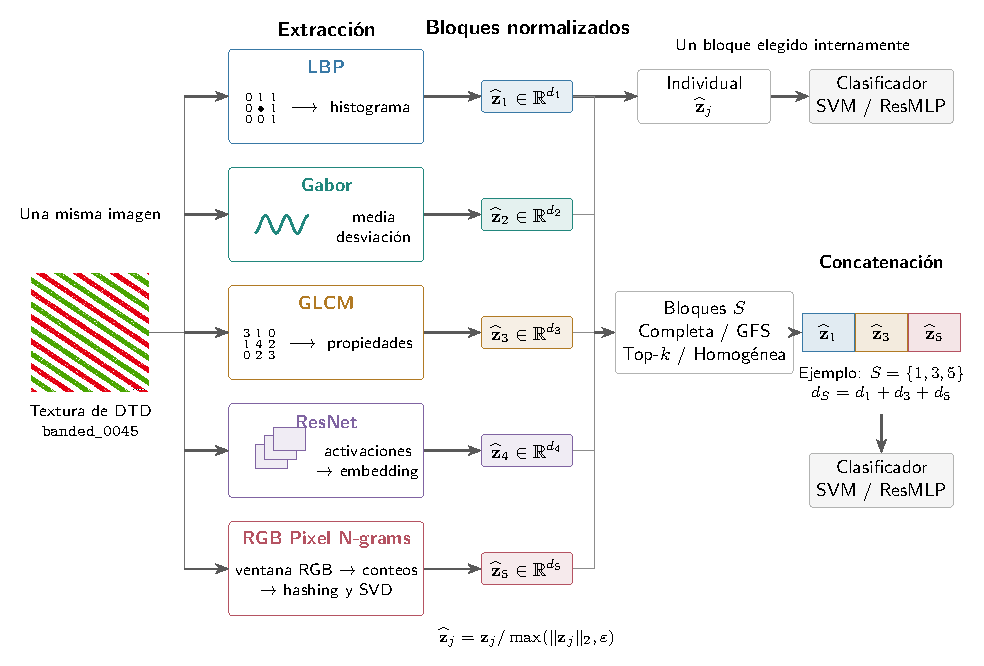
\includegraphics[width=\textwidth]{articulo/borrador_profesor/figures/concatenacion_v02.pdf}
\caption{Extracción y concatenación de descriptores. La misma imagen de DTD se representa mediante cinco ejemplos: patrones locales (LBP), respuestas de filtros (Gabor), coocurrencias (GLCM), una red convolucional (ResNet) y secuencias RGB (N-gramas). Las transformaciones internas se muestran esquemáticamente; no representan mapas de importancia por píxel. Cada rama produce un bloque normalizado que puede utilizarse individualmente o concatenarse con otros. El ejemplo de tres bloques ilustra la unión de coordenadas; cada política determina el subconjunto admisible.}
\label{fig:pipeline}
\end{figure}
\FloatBarrier

\section{Estrategias comparadas}

Las cinco estrategias responden a decisiones sobre la representación que recibe el clasificador. Individual establece el desempeño de un solo bloque; Completa evalúa la unión de toda la biblioteca; Top-$k$ y GFS eligen subconjuntos; Homogénea restringe la procedencia de los bloques a una familia. Se utilizan las mismas denominaciones en método, resultados y estadística:
\begin{enumerate}
\item \textbf{Individual}: descriptor con mayor macro-F1 medio en validación interna.
\item \textbf{Completa}: concatenación de todos los bloques de la biblioteca evaluada.
\item \textbf{Top-$k$}: concatenación de los $k$ descriptores mejor posicionados por su macro-F1 individual interno; $k$ se toma del subconjunto GFS de la misma condición.
\item \textbf{GFS}: subconjunto devuelto por la selección secuencial de bloques.
\item \textbf{Homogénea}: mejor resultado interno de GFS restringido a una familia, con un límite de bloques no mayor que el subconjunto GFS heterogéneo.
\end{enumerate}
Top-$k$ controla la composición bajo el mismo número de bloques que GFS, aunque las dimensiones pueden diferir. No constituye una política independiente de elección de $k$. Homogénea permite estudiar el efecto de restringir la biblioteca a una familia. Todos los comparadores se seleccionan antes de evaluar el test. Los controles aleatorios y las variantes de presupuesto se conservan como análisis auxiliares en los materiales del proyecto.

\section{Espacio de descriptores}

La biblioteca contiene 21 descriptores, agrupados según el tipo de representación. Cada uno constituye un bloque candidato sujeto al mismo criterio de selección. Las
Tablas~\ref{tab:extractores-clasicos} y~\ref{tab:extractores-aprendidos}
identifican la parametrización, los checkpoints y la dimensionalidad de cada
bloque. Las redes preentrenadas se ejecutaron en modo evaluación y sin
ajuste de pesos. En los modelos cargados mediante \texttt{timm} se eliminó la
capa clasificadora (\texttt{num\_classes=0}) y se aplicó el preprocesamiento
asociado al checkpoint. Para ViT, DeiT, Swin, MAE y SigLIP se utilizó la salida
\emph{pooler} cuando estaba disponible y, en caso contrario, el token de
clasificación. Todas las imágenes se convirtieron a RGB.

Los descriptores clásicos se basan en operadores LBP,
Gabor, GLCM y HOG \citep{ojala2002lbp,mehta2016drlbp,jain1991gabor,haralick1979glcm,dalal2005hog}.
Las CNN corresponden a VGG16, ResNet, DenseNet, EfficientNet y ConvNeXt V2
\citep{simonyan2015vgg,he2016resnet,huang2017densenet,tan2019efficientnet,woo2023convnextv2}.
El grupo Transformer incluye ViT, DeiT, Swin y EVA-02
\citep{dosovitskiy2021vit,touvron2021deit,liu2021swin,fang2024eva02}; las
representaciones con preentrenamiento autosupervisado o multimodal se basan en
DINOv2, MAE y SigLIP \citep{oquab2024dinov2,he2022mae,zhai2023siglip}.

\begin{table}[!ht]
\centering
\caption{Seis descriptores basados en patrones, filtros, gradientes y conteos incluidos en la biblioteca. Cada fila constituye un bloque completo.}
\label{tab:extractores-clasicos}
\fontsize{9}{11}\selectfont
\begin{tabular}{@{}lp{7.0cm}p{3.2cm}r@{}}
\toprule
Descriptor & Parametrización & Salida & Dim. \\
\midrule
LBP & multiescala $(P,R)=(8,1),(16,2),(24,3)$; mapeo uniforme invariante a rotación (riu2) & histogramas normalizados & 54 \\
LBP-rot & $P=8$, $R=1$; ocho rotaciones; códigos limitados a $[0,10]$ & histogramas $10\times 8$ & 80 \\
Gabor & cuatro frecuencias 0,1--0,8; seis orientaciones & media y desv. de respuesta real & 48 \\
GLCM & 256 niveles; distancias 1--3; cuatro ángulos; seis propiedades & promedios sobre ángulos & 18 \\
HOG & nueve orientaciones; celda $16^2$; bloque $2^2$; norma L2-Hys & vector HOG & 1.764 \\
N-gramas & ventana vertical $2\times1$; cuantización RGB por 12; 8.192 bins; SVD & vector normalizado & 256 \\
\bottomrule
\end{tabular}
\end{table}

\begin{table}[!ht]
\centering
\caption{Quince representaciones aprendidas congeladas incluidas en la biblioteca. ``Preclas.'' designa la salida inmediatamente anterior al clasificador del backbone.}
\label{tab:extractores-aprendidos}
\fontsize{9}{11}\selectfont
\begin{tabular}{@{}llp{6.5cm}lr@{}}
\toprule
Familia & Descriptor & Checkpoint & Salida & Dim. \\
\midrule
CNN & VGG16 & \texttt{vgg16.tv\_in1k} & preclas. & 4.096 \\
 & ResNet-50 & \texttt{resnet50.a1\_in1k} & preclas. & 2.048 \\
 & ResNet-101 & \texttt{resnet101.a1\_in1k} & preclas. & 2.048 \\
 & DenseNet-121 & \texttt{densenet121.tv\_in1k} & preclas. & 1.024 \\
 & EfficientNet-B0 & \texttt{efficientnet\_b0.ra\_in1k} & preclas. & 1.280 \\
 & ConvNeXt V2-T & \texttt{convnextv2\_tiny.fcmae\_ft\_in22k\_in1k} & preclas. & 768 \\
\midrule
Transformer & ViT-B/16 & \texttt{google/vit-base-patch16-224} & pooler/CLS & 768 \\
 & DeiT-S & \texttt{facebook/deit-small-patch16-224} & pooler/CLS & 384 \\
 & Swin-T & \texttt{microsoft/swin-tiny-patch4-window7-224} & pooler & 768 \\
 & EVA-02 base & \texttt{eva02\_base\_patch14\_224} & preclas. & 768 \\
\midrule
Autosup./multimodal & DINOv2-S & \texttt{vit\_small\_patch14\_dinov2.lvd142m} & preclas. & 384 \\
 & DINOv2-B & \texttt{vit\_base\_patch14\_dinov2.lvd142m} & preclas. & 768 \\
 & DINOv2-L & \texttt{vit\_large\_patch14\_dinov2.lvd142m} & preclas. & 1.024 \\
 & MAE-B & \texttt{facebook/vit-mae-base} & pooler/CLS & 768 \\
 & SigLIP-B & \texttt{google/siglip-base-patch16-224} & pooler/CLS & 768 \\
\bottomrule
\end{tabular}
\end{table}

Los descriptores clásicos se calcularon en escala de grises con la implementación de scikit-image: LBP, LBP-rot, Gabor y GLCM sobre imágenes redimensionadas a $256\times256$, y HOG sobre $128\times128$. LBP-rot designa la implementación propia registrada como \texttt{drlbp} en los archivos experimentales: aplica LBP con mapeo \texttt{ror} a ocho rotaciones y concatena diez bins por rotación en el intervalo $[0,10]$. Los códigos fuera de ese intervalo se descartan; por tanto, es un histograma restringido, no una reproducción del DRLBP de Mehta y Egiazarian \citep{mehta2016drlbp}. Los 21 vectores concatenados suman 19.884 dimensiones. Las características fijas y los conteos por imagen se almacenaron junto con etiquetas, orden de muestras y hashes de procedencia; las transformaciones aprendidas se ajustaron dentro de cada partición de entrenamiento. El estudio evalúa la selección y concatenación de bloques con extractores de imagen congelados y transformaciones ajustadas dentro del entrenamiento; no compara estrategias de \emph{fine-tuning}.

RGB Pixel N-grams \citep{paiva2023rgb} utiliza ventanas verticales de $2\times1$ píxeles con paso 1 sobre la imagen RGB en su resolución original. Cada canal se cuantiza mediante $q(v)=\lfloor v/12\rfloor$; los seis valores se codifican en base 22, recorriendo las dos posiciones de R, G y B. Los conteos se agrupan por el resto del código dividido por 8.192 y se comprimen mediante TruncatedSVD aleatorizado (256 componentes, cinco iteraciones y semilla de la condición). SVD se ajusta exclusivamente con el entrenamiento de cada partición interna y se reajusta sobre el entrenamiento externo para la evaluación final. El vector se normaliza con $L_2$ antes de concatenarlo. Esta parametrización comprimida se identifica como N-gramas + SVD y constituye una familia propia para la selección Homogénea.

\section{Greedy Forward Selection}

GFS se utiliza como un método \emph{wrapper}: los subconjuntos se valoran mediante el propio clasificador y exclusivamente dentro de la validación interna, como requieren los diseños de selección que separan búsqueda y evaluación externa \citep{kohavi1997wrappers,guyon2003feature}. La búsqueda comienza con un conjunto vacío. En el paso $t$, evalúa cada descriptor aún no seleccionado al añadirlo al subconjunto vigente y elige el candidato con mayor macro-F1 medio en la validación interna:
\begin{equation}
 j_t=\arg\max_{j\notin S_{t-1}}\widehat{F}_{1,\mathrm{inner}}(S_{t-1}\cup\{j\}),
 \qquad S_t=S_{t-1}\cup\{j_t\}.
 \label{eq:gfs}
\end{equation}
La búsqueda se limita a $k\leq 8$. Se detiene cuando la mejora respecto del paso anterior es menor que 0,001 durante dos pasos consecutivos, pero devuelve el mejor paso histórico, no necesariamente el último. Los empates se resuelven de forma determinista mediante el nombre del extractor. Todas las evaluaciones candidatas utilizan únicamente muestras pertenecientes al entrenamiento externo.

La Figura~\ref{fig:gfs-pasos} representa el mecanismo general de GFS. En cada ronda se comparan únicamente los bloques aún disponibles dentro de los folds internos; el bloque elegido se incorpora al subconjunto y el test externo permanece fuera de esa decisión.

\begin{figure}[!ht]
\centering
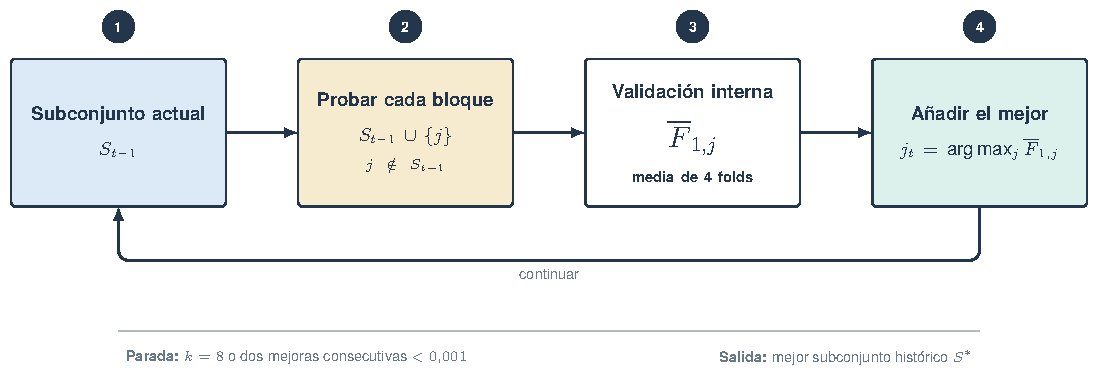
\includegraphics[width=\textwidth]{articulo/borrador_profesor/figures/gfs_pasos.pdf}
\caption{Mecanismo de Greedy Forward Selection sobre bloques completos. En cada paso se elige el bloque que maximiza el macro-F1 medio de la validación interna; el test externo se utiliza únicamente tras cerrar el subconjunto.}
\label{fig:gfs-pasos}
\end{figure}
\FloatBarrier

La Tabla~\ref{tab:config-gfs} concentra los parámetros de búsqueda, comunes a ambos clasificadores.

\begin{table}[!b]
\centering
\caption{Configuración de la selección GFS en el flujo general.}
\label{tab:config-gfs}
\fontsize{9}{11}\selectfont
\begin{tabular}{lp{8.4cm}}
\toprule
Elemento & Configuración \\
\midrule
Unidad de selección & Bloque completo generado por un extractor \\
Candidatos & 21 bloques \\
Criterio interno & Macro-F1 medio en cuatro folds estratificados y agrupados \\
Presupuesto & Hasta $k=8$ bloques \\
Parada & Dos mejoras consecutivas menores que 0,001; se devuelve el mejor paso histórico \\
Empates & Nombre del extractor, en orden determinista \\
Información excluida & Test externo y sus etiquetas durante toda la selección \\
\bottomrule
\end{tabular}
\end{table}
\FloatBarrier


\section{Conjuntos de datos y control de integridad}

Antes del análisis se construyó un manifiesto por dataset y se verificaron etiquetas, orden de muestras, dimensiones, valores finitos y grupos de dependencia. Se utilizaron DTD, FMD, CUReT y Outex. Sus particiones se describen a continuación; los cuatro datasets integran el análisis estadístico principal.

DTD contiene 5.640 imágenes de texturas en condiciones no controladas y proporciona diez particiones oficiales de entrenamiento, validación y prueba \citep{cimpoi2014dtd}. En cada partición se unieron entrenamiento y validación para ejecutar la selección interna, mientras que el test oficial se reservó para una única evaluación. Los duplicados byte-idénticos que cruzaban roles fueron retirados del conjunto de entrenamiento, conservando intacta la evaluación.

FMD reúne 1.000 fotografías de diez categorías de materiales \citep{sharan2013fmd}. Las características fijas y los conteos por imagen se obtuvieron desde las imágenes oficiales en un orden canónico. Cada imagen presentó un hash único y se utilizó como unidad de agrupación. La evaluación externa empleó cinco folds estratificados y agrupados, repetidos con semillas 42, 123 y 2026.

Outex contiene 1.360 BMP RGB de $128\times128$ píxeles, organizados en 68 clases balanceadas. La auditoría verificó archivos legibles, IDs continuos 000000--001359, ausencia de duplicados y la partición oficial de 680 imágenes de entrenamiento y 680 de prueba, con diez muestras de cada clase en cada lado \citep{ojala2002outex}. Todos los bloques respetan el orden de las 1.360 muestras del manifiesto oficial. Este es el único conjunto Outex utilizado en los resultados del artículo.

Para CUReT se utilizó la distribución gris recortada de 61 materiales, con 92 condiciones compartidas por clase \citep{varma2003filter}. Cada condición constituye un grupo para impedir que la misma configuración de adquisición aparezca a ambos lados de una partición. Se definieron dos mitades complementarias deterministas de 46 condiciones: A para selección y entrenamiento con B como test, y la dirección inversa. Esta asignación reproduce de manera transparente el tamaño 46/46 publicado, pero no se presenta como el split histórico exacto. Debido a que las dos direcciones son complementarias y dependientes, sus resultados se interpretarán descriptivamente.

\section{Clasificadores}

Se emplearon dos clasificadores con sesgos diferentes. La SVM lineal se implementa con \texttt{LinearSVC} de scikit-learn: $C=1$, ponderación balanceada por clase, pérdida \emph{squared hinge}, regularización $L_2$, esquema uno-contra-el-resto, tolerancia $10^{-4}$ y un máximo de 10.000 iteraciones.

Se denomina ResMLP a la MLP residual implementada para este estudio sobre vectores de características; no es una reproducción del modelo de imágenes del mismo nombre \citep{touvron2021resmlp}. Proyecta la entrada a 256 unidades y aplica tres bloques residuales, normalización de capa, activaciones GELU, \emph{dropout} de 0,1 y una salida multiclase. Se entrena con entropía cruzada y AdamW, tasa de aprendizaje $10^{-3}$, decaimiento de pesos $10^{-4}$, lotes de 256 muestras y un máximo de 100 épocas. La parada se basa en la pérdida media de entrenamiento: tras diez épocas sin una disminución mayor que $10^{-4}$, se detiene y restaura el mejor estado registrado. No utiliza el test ni una validación adicional para elegir la época. Las semillas se fijan para NumPy y PyTorch; cuando está disponible, la red se ejecuta en GPU.

\section{Configuración experimental y protocolo anidado}

La selección interna utiliza cuatro folds estratificados y agrupados. En DTD se ejecuta dentro de la unión \emph{train+val} de cada split oficial; en FMD dentro del entrenamiento de cada uno de los 15 folds externos; y en CUReT dentro de la mitad de 46 condiciones asignada al entrenamiento. En Outex, las cinco estrategias restringen los cuatro folds internos a las 680 imágenes del entrenamiento oficial. Después de seleccionar el subconjunto y los comparadores, cada modelo se ajusta con todo el entrenamiento externo y se evalúa una sola vez en el test correspondiente. Se verifica programáticamente que ningún grupo aparezca en entrenamiento y prueba.



\section{Análisis estadístico}\label{sec:analisis-estadistico}

El análisis utiliza rankings de Friedman y Quade, contrastes globales y comparaciones por pares con ajuste de Holm, siguiendo una organización empleada en clasificación de texturas \citep{paiva2023rgb}. Los cálculos se realizaron con los paquetes Java ControlTest y MultipleTest distribuidos con el tutorial de pruebas no paramétricas \citep{derrac2011practical}.

La exactitud es la proporción de imágenes clasificadas correctamente. Macro-F1 promedia el F1 de las $C$ clases con igual peso: $\mathrm{macro\mbox{-}F1}=C^{-1}\sum_{c=1}^{C}2TP_c/(2TP_c+FP_c+FN_c)$, donde $TP_c$, $FP_c$ y $FN_c$ son los verdaderos positivos, falsos positivos y falsos negativos de la clase $c$. Esta media evita que la contribución de una clase dependa directamente de su número de muestras.

Macro-F1 es la métrica primaria. Para cada dataset se promedian primero las condiciones externas de cada clasificador y después los dos clasificadores con igual peso. Así se obtienen cuatro bloques, uno por dataset, y cinco estrategias. No se tratan las particiones repetidas ni los dos clasificadores de una misma base como problemas independientes. Se adopta $\alpha=0{,}05$ y Holm se aplica a la familia de diez pares posibles mediante comparaciones de rangos basadas en Friedman; estos valores no son contrastes post hoc de Quade. Se reportan todas las comparaciones, incluidas las que no rechazan la hipótesis nula. Los valores ajustados se acotan a 1 para su presentación.

La exactitud se reporta como métrica descriptiva secundaria sobre las mismas condiciones. La media y la desviación estándar entre particiones describen la variación observada, pero no convierten las particiones dependientes en réplicas independientes. La ausencia de significancia no demuestra equivalencia entre estrategias.

\newpage
\chapter{Resultados del estudio anidado}\label{sec:resultados-experimentales}

\section{Resultados principales: desempeño y descriptor individual}

La Tabla~\ref{tab:resultados-confirmatorios} compara las cinco estrategias con la biblioteca de 21 descriptores. Individual corresponde a una política de selección interna: el descriptor elegido puede cambiar entre particiones. El panel B identifica esos descriptores y sus frecuencias, evitando atribuir la media a un único extractor cuando hubo varios. La Tabla~\ref{tab:accuracy} presenta la exactitud bajo el mismo protocolo.

\begin{resulttable}
\centering\fontsize{9}{11}\selectfont\setlength{\tabcolsep}{3.6pt}
\caption{Macro-F1 externo de las cinco estrategias con la biblioteca de 21 descriptores. Media y desviación estándar entre particiones; Outex tiene un único split. El máximo de cada fila se destaca sin implicar significancia estadística.}
\label{tab:resultados-confirmatorios}
\textbf{Panel A: macro-F1 externo}\par\smallskip
\begin{tabular}{@{}llccccc@{}}
\toprule
Dataset & Clasif. & Individual & Completa & Top-$k$ & GFS & Homogénea \\
\midrule
DTD & SVM & $0{,}8426\,\pm\,0{,}0109$ & $0{,}8629\,\pm\,0{,}0080$ & $0{,}8684\,\pm\,0{,}0080$ & $\mathbf{0{,}8694}\,\pm\,0{,}0096$ & $0{,}8606\,\pm\,0{,}0086$ \\
DTD & ResMLP & $0{,}8373\,\pm\,0{,}0089$ & $0{,}8608\,\pm\,0{,}0100$ & $0{,}8648\,\pm\,0{,}0084$ & $\mathbf{0{,}8660}\,\pm\,0{,}0095$ & $0{,}8611\,\pm\,0{,}0060$ \\
FMD & SVM & $0{,}9726\,\pm\,0{,}0150$ & $0{,}9644\,\pm\,0{,}0174$ & $\mathbf{0{,}9820}\,\pm\,0{,}0105$ & $0{,}9766\,\pm\,0{,}0135$ & $0{,}9789\,\pm\,0{,}0122$ \\
FMD & ResMLP & $0{,}9690\,\pm\,0{,}0133$ & $0{,}9518\,\pm\,0{,}0203$ & $0{,}9753\,\pm\,0{,}0140$ & $\mathbf{0{,}9783}\,\pm\,0{,}0123$ & $0{,}9773\,\pm\,0{,}0109$ \\
CUReT & SVM & $0{,}9948\,\pm\,0{,}0028$ & $\mathbf{0{,}9989}\,\pm\,0{,}0015$ & $0{,}9989\,\pm\,0{,}0010$ & $0{,}9988\,\pm\,0{,}0008$ & $0{,}9989\,\pm\,0{,}0010$ \\
CUReT & ResMLP & $0{,}9971\,\pm\,0{,}0030$ & $\mathbf{0{,}9993}\,\pm\,0{,}0010$ & $0{,}9986\,\pm\,0{,}0015$ & $0{,}9980\,\pm\,0{,}0013$ & $0{,}9982\,\pm\,0{,}0015$ \\
Outex & SVM & $0{,}9066$ & $\mathbf{0{,}9674}$ & $0{,}9441$ & $0{,}9610$ & $0{,}9307$ \\
Outex & ResMLP & $0{,}9476$ & $0{,}9537$ & $0{,}9607$ & $\mathbf{0{,}9715}$ & $0{,}9306$ \\
\bottomrule
\end{tabular}

\par\medskip\textbf{Panel B: descriptor Individual seleccionado}\par\smallskip
\label{tab:individual-identidad}
\begin{tabular}{@{}lll@{}}
\toprule
Dataset & Clasificador & Descriptor (frecuencia) \\
\midrule
DTD & SVM & SigLIP-B (8/10); DINOv2-L (2/10) \\
DTD & ResMLP & SigLIP-B (10/10) \\
FMD & SVM & SigLIP-B (15/15) \\
FMD & ResMLP & SigLIP-B (15/15) \\
CUReT & SVM & DINOv2-L (2/2) \\
CUReT & ResMLP & DINOv2-S (1/2); DINOv2-L (1/2) \\
Outex & SVM & DINOv2-L (1/1) \\
Outex & ResMLP & N-gramas + SVD (1/1) \\
\bottomrule
\end{tabular}
\par\smallskip{\footnotesize Frecuencias de selección interna; cuando cambia el descriptor, la media del panel A reúne esas elecciones.}
\end{resulttable}
\FloatBarrier

\begin{resulttable}
\centering\fontsize{8}{10}\selectfont\setlength{\tabcolsep}{3.0pt}
\caption{Exactitud externa de cinco estrategias con la biblioteca común de 22 descriptores, incluidos RGB N-gramas + SVD y BEiTv2-B. Se muestran medias entre condiciones externas; Outex tiene un único split oficial.}
\label{tab:accuracy}
\begin{tabular}{@{}llccccc@{}}
\toprule
Dataset & Clasif. & Individual & Completa & Top-$k$ & GFS & Homogénea \\
\midrule
DTD & SVM & $0{,}8448$ & $0{,}8654$ & $0{,}8714$ & $\mathbf{0{,}8716}$ & $0{,}8621$ \\
DTD & ResMLP & $0{,}8382$ & $0{,}8635$ & $\mathbf{0{,}8652}$ & $0{,}8651$ & $0{,}8626$ \\
FMD & SVM & $0{,}9727$ & $0{,}9647$ & $\mathbf{0{,}9820}$ & $0{,}9767$ & $0{,}9790$ \\
FMD & ResMLP & $0{,}9690$ & $0{,}9563$ & $0{,}9740$ & $\mathbf{0{,}9783}$ & $0{,}9773$ \\
CUReT & SVM & $0{,}9948$ & $\mathbf{0{,}9989}$ & $\mathbf{0{,}9989}$ & $0{,}9988$ & $\mathbf{0{,}9989}$ \\
CUReT & ResMLP & $0{,}9971$ & $\mathbf{0{,}9991}$ & $0{,}9984$ & $0{,}9986$ & $0{,}9982$ \\
Outex & SVM & $0{,}9103$ & $\mathbf{0{,}9662}$ & $0{,}9441$ & $0{,}9603$ & $0{,}9324$ \\
Outex & ResMLP & $0{,}9485$ & $0{,}9456$ & $0{,}9662$ & $\mathbf{0{,}9721}$ & $0{,}9338$ \\
Soil & SVM & $0{,}9044$ & $\mathbf{0{,}9281}$ & $0{,}9225$ & $0{,}9152$ & $0{,}9126$ \\
Soil & ResMLP & $0{,}9044$ & $\mathbf{0{,}9184}$ & $0{,}9181$ & $0{,}9170$ & $0{,}9135$ \\
KTH-TIPS2-b & SVM & $0{,}9415$ & $\mathbf{0{,}9609}$ & $0{,}9419$ & $0{,}9112$ & $0{,}9293$ \\
KTH-TIPS2-b & ResMLP & $0{,}9099$ & $\mathbf{0{,}9499}$ & $0{,}9346$ & $0{,}9219$ & $0{,}9165$ \\
\bottomrule
\end{tabular}
\end{resulttable}
\FloatBarrier

\begin{resulttable}
\centering\fontsize{8}{10}\selectfont\setlength{\tabcolsep}{3.0pt}
\caption{Dimensión media de las representaciones usadas en la evaluación externa con 22 descriptores.}
\label{tab:dimensiones}
\begin{tabular}{@{}llrrrrr@{}}
\toprule
Dataset & Clasif. & Individual & Completa & Top-$k$ & GFS & Homogénea \\
\midrule
DTD & SVM & $819{,}2$ & $20652{,}0$ & $4480{,}0$ & $5390{,}4$ & $2496{,}0$ \\
DTD & ResMLP & $768{,}0$ & $20652{,}0$ & $4211{,}2$ & $4626{,}4$ & $2598{,}4$ \\
FMD & SVM & $768{,}0$ & $20652{,}0$ & $2969{,}6$ & $2687{,}5$ & $2338{,}1$ \\
FMD & ResMLP & $768{,}0$ & $20652{,}0$ & $3404{,}8$ & $3077{,}5$ & $2218{,}7$ \\
CUReT & SVM & $1024{,}0$ & $20652{,}0$ & $3328{,}0$ & $4402{,}0$ & $2944{,}0$ \\
CUReT & ResMLP & $704{,}0$ & $20652{,}0$ & $2176{,}0$ & $2880{,}0$ & $1856{,}0$ \\
Outex & SVM & $1024{,}0$ & $20652{,}0$ & $7808{,}0$ & $6784{,}0$ & $3712{,}0$ \\
Outex & ResMLP & $256{,}0$ & $20652{,}0$ & $6016{,}0$ & $3346{,}0$ & $2176{,}0$ \\
Soil & SVM & $768{,}0$ & $20652{,}0$ & $4898{,}1$ & $3709{,}9$ & $2184{,}5$ \\
Soil & ResMLP & $768{,}0$ & $20652{,}0$ & $5529{,}6$ & $4415{,}6$ & $2235{,}7$ \\
KTH-TIPS2-b & SVM & $832{,}0$ & $20652{,}0$ & $1280{,}0$ & $960{,}0$ & $960{,}0$ \\
KTH-TIPS2-b & ResMLP & $672{,}0$ & $20652{,}0$ & $1600{,}0$ & $1440{,}0$ & $928{,}0$ \\
\bottomrule
\end{tabular}
\par\smallskip{\footnotesize Completa tiene siempre 20.652 coordenadas; las otras estrategias pueden elegir subconjuntos distintos entre particiones.}
\end{resulttable}
\FloatBarrier


GFS obtiene mayor macro-F1 medio que Individual en las ocho configuraciones, pero el método con mayor desempeño depende del dataset. Completa alcanza los mayores valores en CUReT y en Outex con SVM; GFS obtiene el mayor valor en Outex con ResMLP. En DTD destaca GFS, mientras que en FMD destacan Top-$k$ con SVM y GFS con ResMLP. Esta comparación describe las medias externas y no implica que cada diferencia sea estadísticamente significativa.

La Tabla~\ref{tab:dimensiones} permite contrastar el desempeño con el tamaño de la representación en las cinco estrategias. La dimensión media de GFS por configuración dataset--clasificador se sitúa entre 2.909,3 y 5.632 componentes, una reducción de entre 71,7\% y 85,4\% respecto de los 19.884 de Completa. Este rango compara las ocho medias, no los extremos de las particiones individuales. La disminución corresponde al vector almacenado y utilizado por el clasificador. No se midió una reducción proporcional de latencia o memoria de extremo a extremo.

\section{Rankings y comparaciones estadísticas}\label{sec:replica-paiva}

Las Tablas~\ref{tab:rankings-comparison} y~\ref{tab:global-tests-comparison} presentan los rankings y los contrastes de la biblioteca de 21 descriptores bajo las dos formas de agregación.

\begin{resulttable}
\centering\fontsize{8.5}{10.5}\selectfont\setlength{\tabcolsep}{3.2pt}
\caption{Rankings medios de macro-F1 con las dos formas de agregación. Menor ranking indica mejor posición relativa.}
\label{tab:rankings-comparison}
\begin{tabular}{@{}lrrrr@{}}
\toprule
Estrategia & Friedman: dataset & Quade: dataset & Friedman: dataset--clasificador & Quade: dataset--clasificador \\
\midrule
Individual & $4{,}750$ & $4{,}800$ & $4{,}625$ & $4{,}611$ \\
Completa & $2{,}750$ & $2{,}800$ & $2{,}875$ & $2{,}944$ \\
Top-$k$ & $2{,}000$ & $2{,}200$ & $2{,}125$ & $2{,}250$ \\
GFS & $2{,}250$ & $1{,}700$ & $2{,}125$ & $1{,}639$ \\
Homogénea & $3{,}250$ & $3{,}500$ & $3{,}250$ & $3{,}556$ \\
\bottomrule
\end{tabular}
\par\smallskip{\footnotesize Dataset: SVM y ResMLP se promedian dentro de cada dataset (cuatro bloques). Dataset--clasificador: se conservan separados (ocho bloques).}
\end{resulttable}
\FloatBarrier

\begin{resulttable}
\centering\fontsize{8.5}{10.5}\selectfont\setlength{\tabcolsep}{4pt}
\caption{Contrastes globales de macro-F1 bajo las dos formas de agregación.}
\label{tab:global-tests-comparison}
\begin{tabular}{@{}llrrr@{}}
\toprule
Agregación & Prueba & Estadístico & gl & $p$ \\
\midrule
Dataset & Friedman & 7,6000 & 4 & 0,1074 \\
Dataset & Quade & 2,8632 & 4,12 & 0,0705 \\
Dataset--clasificador & Friedman & 13,6000 & 4 & 0,0087 \\
Dataset--clasificador & Quade & 5,1248 & 4,28 & 0,0032 \\
\bottomrule
\end{tabular}
\par\smallskip{\footnotesize En la primera agregación se promedian SVM y ResMLP por dataset; en la segunda se mantienen como bloques separados.}
\end{resulttable}
\FloatBarrier

\begin{resulttable}
\centering\fontsize{8.5}{10.5}\selectfont\setlength{\tabcolsep}{4pt}
\caption{Comparaciones frente a Individual: p-values ajustados mediante Holm bajo las dos formas de agregación.}
\label{tab:vs-individual-comparison}
\begin{tabular}{@{}lrr@{}}
\toprule
Comparación & Dataset & Dataset--clasificador \\
\midrule
GFS vs. Individual & $0{,}2281$ & $0{,}0157$ \\
Top-$k$ vs. Individual & $0{,}1391$ & $0{,}0157$ \\
Completa vs. Individual & $0{,}5891$ & $0{,}2149$ \\
Homogénea vs. Individual & $1{,}0000$ & $0{,}5739$ \\
\bottomrule
\end{tabular}
\par\smallskip{\footnotesize Dataset utiliza cuatro bloques; dataset--clasificador utiliza ocho. En ambos casos se aplica Holm sobre la familia de diez comparaciones.}
\end{resulttable}
\FloatBarrier


La Tabla~\ref{tab:vs-individual-comparison} presenta las mismas cuatro comparaciones frente a Individual en paralelo. Al promediar SVM y ResMLP por dataset, los valores ajustados con Holm son 0,2281 para GFS y 0,1391 para Top-$k$; al mantener separados los clasificadores, ambos alcanzan 0,0157. Completa y Homogénea obtienen 0,2149 y 0,5739 en la segunda organización. Como magnitud descriptiva, las diferencias absolutas de macro-F1 de GFS frente a Individual, promediando ambos clasificadores, son 0,0277 en DTD, 0,0066 en FMD, 0,0024 en CUReT y 0,0392 en Outex.

Las dos organizaciones responden a preguntas distintas: la primera resume el comportamiento medio por dataset y la segunda permite observar si el efecto se mantiene por clasificador. Las ocho filas desagregadas reutilizan los mismos datasets e imágenes, por lo que sus resultados deben interpretarse junto con la estructura de dependencia del protocolo. Los procedimientos adicionales y sus salidas Java se conservan en los materiales de reproducibilidad.

\newpage
\chapter{Discusión}\label{sec:discusion}

La comparación muestra que concatenar descriptores puede mejorar el desempeño respecto de elegir un único bloque, pero el beneficio depende de la composición y del dominio. En DTD y FMD, seleccionar un subconjunto ofrece resultados competitivos frente a utilizar toda la biblioteca. En CUReT, Completa alcanza los mayores valores; en Outex, la mejor estrategia depende del clasificador: Completa con SVM y GFS con ResMLP. La concatenación completa mejora descriptivamente frente a Individual en tres de los cuatro datasets al promediar los clasificadores, pero pierde desempeño en FMD. Seleccionar bloques ofrece una alternativa de menor dimensión, cuyo resultado depende de su composición. Este patrón es compatible con distintas combinaciones de información complementaria y redundante; el diseño no mide directamente esa redundancia ni identifica un mecanismo causal.

Las pruebas de Friedman, Quade y Holm moderan la interpretación de las ventajas descriptivas de la biblioteca de 21 descriptores. Con cuatro datasets no se obtuvo evidencia suficiente para afirmar una superioridad global. Esto no demuestra igualdad de rendimiento; delimita lo que sostienen los contrastes realizados.

\section{Limitaciones}

GFS es una búsqueda local y no garantiza el subconjunto óptimo. Top-$k$ hereda su presupuesto de bloques, por lo que compara composiciones bajo un $k$ compartido. Individual se elige internamente y no representa al descriptor con mejor resultado a posteriori en el test. Las particiones de DTD y FMD reutilizan imágenes, CUReT presenta dos direcciones complementarias y Outex tiene una sola partición. El número de datasets limita la precisión y la generalización de la inferencia multibase. No se realizó un cálculo de tamaño muestral a priori ni se presentan intervalos de confianza de generalización a nuevos datasets. Las desviaciones entre particiones describen la variabilidad observada; no estiman esa incertidumbre tratando folds dependientes como réplicas independientes.

Los descriptores clásicos se calcularon sobre escala de grises, mientras las redes y RGB Pixel N-grams utilizan RGB; en CUReT las imágenes de origen son grises. Además, los corpus de preentrenamiento de los modelos podrían solaparse con imágenes de los benchmarks; ese solapamiento no fue auditado. El agrupamiento de conteos y la reducción de dimensión pueden perder información. El histograma restringido de LBP-rot también descarta códigos; la comparación incluye esa implementación específica y no permite extraer conclusiones sobre el DRLBP original. Los resultados dependen de la parametrización especificada. No se dispone de mediciones homogéneas de latencia y memoria para atribuir ahorro de cómputo a la reducción dimensional.

\newpage
\chapter{Conclusión}\label{sec:conclusion}

Este trabajo estudió la concatenación de descriptores como una elección entre representaciones individuales, completas y seleccionadas. La evaluación completa reunió 21 descriptores, cuatro datasets y dos clasificadores bajo un protocolo que separa selección interna y evaluación externa. Las cinco estrategias se compararon mediante macro-F1 y exactitud, con rankings de Friedman y Quade y comparaciones por pares ajustadas mediante Holm.

Los resultados muestran beneficios descriptivos de combinar representaciones y reducciones dimensionales al seleccionar subconjuntos. Ninguna estrategia obtiene el mayor desempeño en todos los dominios. Los contrastes principales entre cuatro datasets no permiten afirmar una superioridad estadística general de GFS, Top-$k$, Completa o Homogénea frente a Individual.

La elección de una representación debe considerar el desempeño externo y la dimensionalidad bajo un protocolo común. Como siguientes pasos se plantea ampliar la diversidad de datasets, estudiar el efecto de la normalización y medir de forma homogénea el costo de extracción y clasificación.


% ============================================================
% BIBLIOGRAFÍA
% ============================================================
\newpage
\bibliographystyle{unsrtnat}
\bibliography{articulo/borrador_profesor/references}

\end{document}
